\documentclass[parskip=full]{scrartcl}
\usepackage[utf8]{inputenc} % use utf8 file encoding for TeX sources
\usepackage[T1]{fontenc}    % avoid garbled Unicode text in pdf
\usepackage[german]{babel}  % german hyphenation, quotes, etc
\usepackage{hyperref}       % detailed hyperlink/pdf configuration
\hypersetup{                % ‘texdoc hyperref‘ for options
pdftitle={Pflichtenheft zu ***},%
bookmarks=true,%
}
\usepackage{graphicx}       % provides commands for including figures
\usepackage{csquotes}       % provides \enquote{} macro for "quotes"
\usepackage[nonumberlist]{glossaries}     % provides glossary commands
\usepackage{enumitem}

\makenoidxglossaries
%
% % Glossareinträge
%
\newglossaryentry{Nutzer}
{
	name=Nutzer,
	description={Ein Individuum, das die Kriterien der Zielgruppe erfüllt und das Produkt bewusst verwendet}
}

\newglossaryentry{Mobiltelefon}
{
	name=Mobiltelefon des Nutzers,
    plural=Mobiltelefon,
	description={Das Mobiltelefon, mit dem \gls{Nutzer} das Produkt verwendet. Es wird angenommen, dass ein Nutzer das Produkt mit genau einem Mobiltelefon verwendet. Sagt nichts darüber aus, ob der Nutzer der Eigentümer des Mobiltelefons ist, auch wenn normalerweise der Fall sein wird}
}

\newglossaryentry{Kunde}
{
	name=Kunde,
	plural=Kunden,
	description={(Zahlende) Teilnehmer einer oder mehrerer Seminarveranstaltung/en}
}

\newglossaryentry{Zielbild}
{
	name=Zielbild,
	plural=Zielbilder,
	description={Das Resultat, welches das Produkt liefert, nachdem es ein Bild oder mehrere Bilder zu einem einzigen neuen Bild verarbeitet hat}
}

\newglossaryentry{Einzelbepreisung}
{
	name=Einzelbepreisung,
	plural=Einzelbepreisungen,
	description={Bezahlmodell, in dem die Kosten jeder Bildverarbeitung des Produkts einzeln berechnet und bezahlt werden}
}

\newglossaryentry{Monatsabonnement}
{
	name=Monatsabonnement,
	plural=Monatsabonnements,
	description={Bezahlmodell, in dem ein Pauschalpreis für alle Bildverarbeitungen des Produkts in einem Monat bezahlt wird. Mit einer einmaligen Zahlung sind dann die Kosten alle Bildverarbeitungen in den folgenden 30 Tagen gedeckt}
}

\newglossaryentry{Bild}
{
	name=Bild,
	plural=Bilder,
	description={Eine Datei in einem der Bildformate JPG/JPEG oder PNG}
}

\newglossaryentry{Zahlungsmethode}
{
	name=Zahlungsmethode,
	plural=Zahlungsmethoden,
	description={Beschreibt das Mittel und die Art und Weise, mit dem und in der bezahlt wird. (z.B. \textit{PayPal Direktzahlung} oder \textit{SEPA Lastschriftverfahren})}
}

\newglossaryentry{Zahlungsdienstleister}
{
	name=Zahlungsdienstleister,
	description={Ein Geldinstitut oder ähnliches, das eine öffentlich zugängliche \gls{Zahlungsmethode} anbietet}
}

\newglossaryentry{Zahlungsdetails}
{
	name=Zahlungsdetails,
	description={Die Menge der Informationen über die \gls{Zahlungsmethode}, die der \gls{Zahlungsdienstleister} der Zahlungsmethode benötigt, um den \gls{Nutzer}, der die Zahlung in Auftrag gibt, zu identifizieren}
}

\newglossaryentry{GUI}
{
	name=Nutzeroberfläche,
	plural=Nutzeroberflächen,
	description={Graphische Schnittstelle, über die ein \gls{Nutzer} mit dem Produkt interagieren kann}
}

\title{Pflichtenheft zu ***}
\author{Lennart Großkreutz, Timo Weberruß, Corvin Navarro Ecker, \\ Tobias Gröger, Marius Baden}

\newcommand{\paragraphashead}[1]{\paragraph{#1}\mbox{}\\\\}

\begin{document}

\maketitle

%
% % Hier beginnt die Gliederung des Lastenhefts
%
\section{Zielbestimmung}
Deutschsprachige Mobiltelefonbesitzer sollen mithilfe des Produkts in der Lage sein \glspl{Bild}, die auf ihrem \glspl{Mobiltelefon} gespeichert sind, zu bearbeiten. Die Bearbeitung dreht sich hauptsächlich darum, den Bildhintergrund zu verändern. Der \gls{Nutzer} wird mit einer \gls{GUI} durch den Prozess geleitet.

\section{Produkteinsatz}
Das Produkt soll über den \textit{Apple App Store}, \textit{Google Play} und weitere gängige App Stores kostenlos erhältlich sein. Es dient dazu persönliche Bilder des \gls{Nutzer}s nach den Wünschen des Nutzers zu verändern. Außerdem berechnet das Produkt die Kosten der Bildbearbeitung und kontrolliert, dass nur zahlende Nutzer vom Produkt bearbeitete Bilder speichern können. 

Zielgruppe: Menschen, die Zugang zu einem Mobiltelefon besitzen und die deutsche Sprache lesen können.

Plattform: Mobiltelefon mit \textit{iOS 7}, \textit{Android 6 Marshmallow} oder einer Nachfolgerversion der beiden Betriebssysteme.

\section{Funktionale Anforderungen}
\begin{itemize}[nosep]
\item[FA10] Entfernen einer angegebenen Farbe aus dem Hintergrund eines Bilds A und Ersetzen des entfernten Teils aus Bild A mit einem anderen Bild B. Anzeigen des so aus Bild A und Bild B zusammengesetzten \gls{Zielbild}s.
\item[FA11] Einfügen von Text in das Zielbild (optional), Definieren der gewünschten Skalierung des Zielbilds (verpflichtend) und Wahl der Positionierung von Bild A gegenüber Bild B (verpflichtend) als Zusatzoptionen zu /FA10/.
\item[FA20] Berechnung der Kosten der verschiedenen Kaufoptionen abhängig davon, ob das Bild bereits mit dem Produkt bearbeitet wurde. Das Produkt bietet sowohl eine \gls{Einzelbepreisung} als auch ein \gls{Monatsabonnement} als Kaupfoptionen an.
\item[FA21] Sowohl Abfragen der \gls{Zahlungsmethode} und \gls{Zahlungsdetails} vom Nutzer als auch Übermittlung der Anweisung zur Transaktion an den \gls{Zahlungsdienstleister}.
\item[FA22] Überprüfen, ob der Zahlungsdienstleister eine Transaktion bestätigt hat.
\item[FA30] Speicherung des durch /FA10/ entstandenen Zielbilds auf dem Mobiltelefon des Nutzers nur falls der Nutzer dafür eine Kaufoption aus /FA20/ gewählt und diese Kaufoption bezahlt hat.
\item[FA31] Hat ein Nutzer bereits - z.B. durch ein Monatsabonnement - im voraus für die Verarbeitung des durch /FA10/ enstandenen Zielbilds bezahlt, so wird ihm bei der Speicherung des Zielbilds durch /FA30/ keine Abfrage zu den Kaufoptionen gestellt.
\item[FA40] Auflisten und Anzeigen der letzen 50 mit dem Produkt erstelleten Bilder.
\item[FA50] Teilen der erstellten Bilder über gängige soziale Netzwerke.

\end{itemize}

\section{Produktdaten}
\begin{itemize}[nosep]
\item[PD10] Von allen Nutzern sind alle Eingabebilder A und B aus /FA10/ und alle Zielbilder aus /FA10/ auf dem Zentral-Server der Pear Corp. zu speichern.
\item[PD20] Für jeden Nutzer sind die durch /FA10/ entstandenen Zielbilder auf seinem Mobiltelefon zu speichern, falls er die Bedingung in /FA30/ erfüllt.
\item[PD30] Falls ein Nutzer sich für die Kaufoption Monatsabonnement entscheidet, dann sind relevante Daten über die Zahlungsmethode und die Zahlungsdetails des Nutzers zu speichern.
\end{itemize}

\section{Nichtfunktionale Anforderungen}
\begin{itemize}[nosep]
\item[NF10] Die Bildverarbeitung in /FA10/ findet nicht auf dem Mobiltelefon des Nutzers statt, sondern auf dem Zentral-Server der Pear Corp. Die Ausgangsbilder A und B werden dazu vor der Verarbeitung über das Internet an den Zentral-Server gesendet. Nach erfolgreicher Zahlung in /FA20/ wird das Zielbild über das Internet an das Mobiltelefon des Nutzers gesendet.
\item[NF20] Ein Verarbeitungsvorgang in /FA10/ von den Bilder A und B zum Zielbild darf maximal 1 Sekunde dauern.
\item[NF30] Es müssen bis zu 1.000 Bildverarbeitungen in /FA10/ gleichzeitig durchgeführt werden können. Insbesondere muss dabei die maximale Dauer je Verarbeitung aus /NF20/ eingehalten werden.
\item[NF40] Bei der Funktion /FA40/ darf zwischen dem Aufrufen der Funktion und dem Erscheinen der Bilder auf der Nutzeroberfläche höchstens eine Sekunde vergehen. 
\end{itemize}

\section{Systemmodelle}

\subsection{Szenarien}
\subsubsection{Verarbeiten eines Bildes und Bezahlen per Einzelbepreisung}
John ist aus dem Urlaub am Meer wieder nach Hause zurückgekehrt. Ihm fällt auf, dass er viele Bilder vom Strand und dem Meer im Hintergrund mit seinem Mobiltelefon gemacht hat, aber kein einziges auf dem er selbst zu sehen ist. Seine Frau Alice hat jedoch ein Bild von ihm im Hotel gemacht, wie er vor einer weißen Wand steht. Also öffnet er die iMage-App auf seinem Android Smartphone. Er drückt im Startmenu auf \grqq{}Neues Bild erstellen", woraufhin ihm die Bilder angezeigt werden, die er auf seinem Mobiltelefon gespeichert hat. Er wählt das Bild von ihm im Hotel aus, welches ihm Alice per E-Mail auf sein Mobiltelefon geschickt hat. Dann setzt er als Zielgröße 1920x1080 Pixel und gibt weiß - die Farbe der Wand hinter ihm im Hotel - als zu entfernende Farbe ein. Er lehnt ab Text in das Bild einzufügen. Anschließend werden ihm erneut die auf seinem Mobiltelefon gespeicherten Bilder angezeigt. Diesmal sucht er darunter ein besonders schönes Strandbild aus seinen Urlaubsbilder aus. Er gibt ein, dass das Bild von ihm unten mittig auf dem Hintergrund platziert werden soll und bestätigt seinen Verarbeitungsauftrag. Nun zeigt ihm das Produkt ein Bild an auf dem er aus dem Hotel zu sehen ist. Jedoch befindet sich im Hintergrund nicht mehr die Wand sondern der Strand und das Meer. John ist zufrieden mit dem Ergebnis. Er wählt "Bild abholen\grqq{}  aus. Daraufhin wählt er aus nur dieses Bild für 0,45€ zu bezahlen. Er wählt das SEPA Lastschriftverfahren als Zahlungsmethode und gibt seinen Namen, Bankleitzahl und IBAN ein. Nun kann er das Bild auf seinem Mobiltelefon speichern. Er schließt die App und zeigt das neue Bild seiner Frau auf seinem Mobiltelefon.

\subsection{Anwendungsfälle}
\subsubsection{Seminarorganisation}
\begin{center}
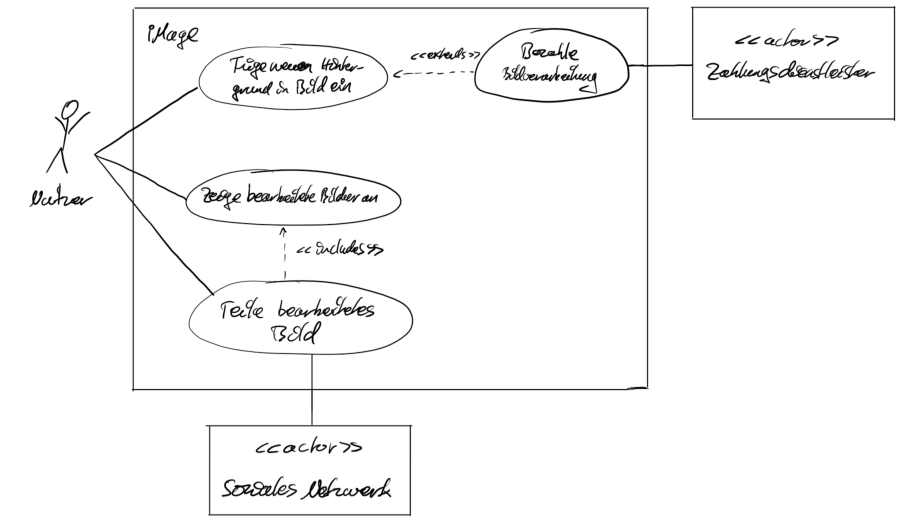
\includegraphics[width=0.8\textwidth]{resources/anwendungsfalldiagramm.pdf}
\end{center}

Akteure: Nutzer, Zahlungsdienstleister, soziales Netzwerk.

Anwendungsfälle: Füge neuen Hintergrund in Bild ein, Zeige bearbeitete Bilder an, Teile bearbeitetes Bild, Bezahle Bildverarbeitung.


\paragraphashead{Anwendungsfall: Füge neuen Hintergrund in Bild ein}
Teilnehmender Akteur
    \begin{itemize}\setlength\itemsep{-1em}
        \item Nutzer
    \end{itemize}
Eingangsaktionen
	\begin{itemize}\setlength\itemsep{-1em}
    	\item Nutzer hat zwei Bilder auf seinem Mobiltelefon gespeichert
        \item Nutzer wählt die Funktion "Neues Bild erstellen" aus
    \end{itemize}
Ausgangsaktionen
	\begin{itemize}\setlength\itemsep{-1em}
        \item Nutzer speichert das Bild auf seinem Mobiltelefon
    \end{itemize}
Ereignisfluss
	\begin{itemize}\setlength\itemsep{-1em}
        \item Der Nutzer wählt ein Vordergrundbild, das auf seinem Mobiltelefon gespeichert ist, aus
        \item Der Nutzer wählt die Größe des Zielbild und die zu entfernende Farbe im Hintergrund aus
        \item  Der Nutzer wählt aus, ob er Text in das Zielbild einfügen will. Sollte das der Fall sein, so gibt er außerdem an, welcher Text eingefügt werden soll und wo er eingefügt werden soll.
        \item Der Nutzer wählt ein Hintergrundbild, das auf seinem Mobiltelefon gespeichert ist, aus
        \item Der Nutzer legt die Positionierung des Vordergrundbilds im Verhältnis zum Hintergrundbild fest
        \item Das Produkt verarbeitet die beiden Bilder entsprechend den Eingaben zum Zielbild
        \item Das Zielbild wird dem Nutzer angezeigt
        \item Falls der Nutzer die Bildverarbeitung nicht im voraus bezahlt hat, zahlt der Nutzer für das Bild (Anwendungsfall "Bezahle Bildverarbeitung").
        \item Der Nutzer speichert das Zielbild auf seinem Mobiltelefon
    \end{itemize}
Spezielle Anforderungen
\begin{itemize}\setlength\itemsep{-1em}
  \item Das Mobiltelefon des Nutzers ist mit dem Internet verbunden
\end{itemize}

\paragraphashead{Anwendungsfall: Bezahle Bildverarbeitung}
Teilnehmender Akteure
    \begin{itemize}\setlength\itemsep{-1em}
        \item Nutzer
        \item Zahlungsdienstleister
    \end{itemize}
Eingangsaktionen
	\begin{itemize}\setlength\itemsep{-1em}
    	\item Das Produkt hat Bilder zu einem Zielbild verarbeitet
        \item Der Nutzer hat für diesen Verarbeitungprozess noch nicht bezahlt
    \end{itemize}
Ausgangsaktionen
	\begin{itemize}\setlength\itemsep{-1em}
        \item Das Produkt erlaubt dem Nutzer das Bild auf seinem Mobiltelefon zu speichern
    \end{itemize}
Ereignisfluss
	\begin{itemize}\setlength\itemsep{-1em}
        \item Der Nutzer wählt Kaufoption aus
        \item Der Nutzer wählt eine \gls{Zahlungsmethode} und gibt seine \gls{Zahlungsdetails} ein
        \item Das Produkt übermittelt die Anweisung des Nutzers zur Transaktion an den Zahlungsdienstleister
         \item Der Zahlungsdienstleister bestätigt die Transaktion
         \item Das Produkt empfängt die Transaktionsbestätigung und schaltet das Zielbild für den Nutzer zum Speichern auf seinem Mobiltelefon frei
    \end{itemize}
Spezielle Anforderungen
\begin{itemize}\setlength\itemsep{-1em}
  \item Das Mobiltelefon des Nutzers ist mit dem Internet verbunden
\end{itemize}

\paragraphashead{Anwendungsfall: Zeige bearbeitete Bilder an}
Teilnehmender Akteur
    \begin{itemize}\setlength\itemsep{-1em}
        \item Nutzer
    \end{itemize}
Eingangsaktionen
	\begin{itemize}\setlength\itemsep{-1em}
    	\item Der Nutzer wählt die Funktion "Bearbeitete Bilder anzeigen" 
    \end{itemize}
Ausgangsaktionen
	\begin{itemize}\setlength\itemsep{-1em}
        \item Das Produkt zeigt dem Nutzer aller Bilder an, die der Nutzer zuletzt mit dem Produkt bearbeitet hat
    \end{itemize}
Ereignisfluss
	\begin{itemize}\setlength\itemsep{-1em}
        \item Das Produkt zeigt dem Nutzer aller Bilder an, die der Nutzer zuletzt mit dem Produkt bearbeitet hat
    \end{itemize}
Spezielle Anforderungen: keine

\paragraphashead{Anwendungsfall: Teile bearbeitetes Bild}
Teilnehmender Akteur
    \begin{itemize}\setlength\itemsep{-1em}
        \item Nutzer
        \item Soziales Netzwerk
    \end{itemize}
Eingangsaktionen
	\begin{itemize}\setlength\itemsep{-1em}
    	\item Der Nutzer hat ein Bild mit dem Produkt bearbeitet
    \end{itemize}
Ausgangsaktionen
	\begin{itemize}\setlength\itemsep{-1em}
        \item Das soziale Netzwerk teilt ein Bild im Namen des Nutzers
    \end{itemize}
Ereignisfluss
	\begin{itemize}\setlength\itemsep{-1em}
    	\item Der Nutzer lässt sich die von ihm zuletzt mit dem Produkt bearbeiteten Bilder anzeigen
        \item Der Nutzer wählt ein zuletzt bearbeites Bild aus
        \item Der Nutzer wählt die Funktion "Über soziales Netzwerk teilen" aus
        \item Der Nutzer wählt ein soziales Netzwerk aus, über das er das ausgewählte Bild teilen möchte
        \item Der Nutzer wird an das soziale Netzwerk weitergeleitet, wo er sich mit einem Konto beim sozialen Netzwerk anmelden kann
        \item Das soziale Netzwerk teilt das Bild im Namen des Nutzers
    \end{itemize}
Spezielle Anforderungen
\begin{itemize}\setlength\itemsep{-1em}
  \item Das Mobiltelefon des Nutzers ist mit dem Internet verbunden
\end{itemize}

\newpage

%
% % Automatisch generiertes Glossar (Latex zwei mal ausführen um Glossar anzuzeigen)
%
%\glsaddall % das sorgt dafür, dass alles Glossareinträge gedruckt werden, nicht nur die verwendeten. Das sollte nicht nötig sein!
\printnoidxglossaries

\end{document}
